\documentclass[border=0pt, 12pt, tikz]{standalone}
\usepackage{pgfplots}

\begin{document}
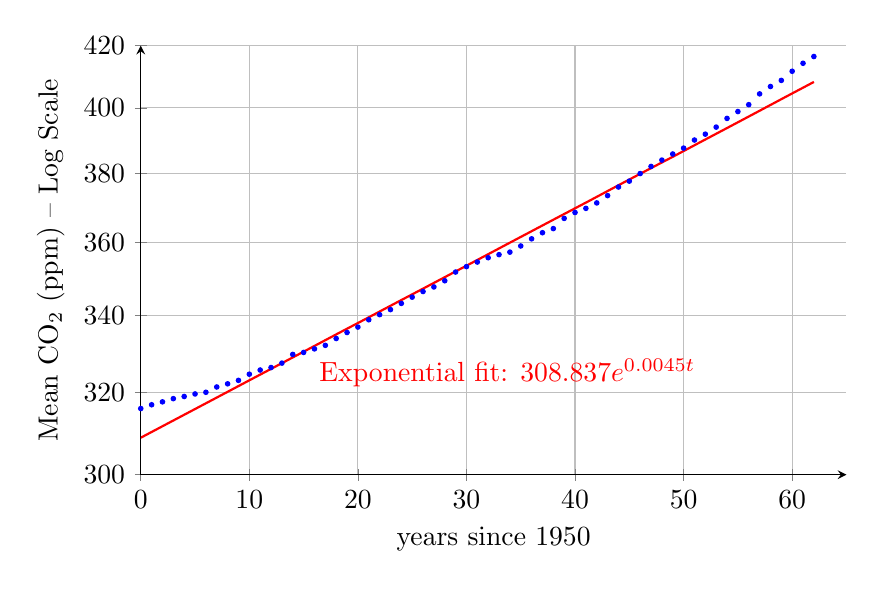
\begin{tikzpicture} 
\begin{axis}%   
[ axis lines = left
, width=300pt
, height=200pt
, ymode = log
, xlabel = {years since 1950}
, ylabel = {Mean CO$_2$ (ppm) -- Log Scale}     
, ymax=420
, ymin=300
, xmax = 65
, xmin = 0
, log ticks with fixed point
, grid = both
, ytick ={300,320, 340, ...,420}
] 
\addplot[color=red, domain=0:62,style=thick]{308.837*exp(0.0045*x)} node[below right,pos=0.25]{Exponential fit: $308.837e^{0.0045t}$}; 

\addplot
[ color = blue
, only marks
, mark = *
, mark options = {scale = 0.4}
% , style = thick
% , mark=none
] coordinates {%
(0,  315.98)
(1,  316.91)
(2,  317.64)
(3,  318.45)
(4,  318.99)
(5,  319.62)
(6,  320.04)
(7,  321.37)
(8,  322.18)
(9,  323.05)
(10, 324.62)
(11, 325.68)
(12, 326.32)
(13, 327.46)
(14, 329.68)
(15, 330.19)
(16, 331.12)
(17, 332.03)
(18, 333.84)
(19, 335.41)
(20, 336.84)
(21, 338.76)
(22, 340.12)
(23, 341.48)
(24, 343.15)
(25, 344.85)
(26, 346.35)
(27, 347.61)
(28, 349.31)
(29, 351.69)
(30, 353.2)
(31, 354.45)
(32, 355.7)
(33, 356.54)
(34, 357.21)
(35, 358.96)
(36, 360.97)
(37, 362.74)
(38, 363.88)
(39, 366.84)
(40, 368.54)
(41, 369.71)
(42, 371.32)
(43, 373.45)
(44, 375.98)
(45, 377.7)
(46, 379.98)
(47, 382.09)
(48, 384.02)
(49, 385.83)
(50, 387.64)
(51, 390.1)
(52, 391.85)
(53, 394.06)
(54, 396.74)
(55, 398.87)
(56, 401.01)
(57, 404.41)
(58, 406.76)
(59, 408.72)
(60, 411.66)
(61, 414.24)
(62, 416.45)
};
\end{axis} 
\end{tikzpicture}
\end{document}